\documentclass[10pt,utf8,presentation]{beamer}

\usepackage[utf8]{inputenc}
\usepackage{default}

\usepackage[T2A]{fontenc}
% \usepackage[russian]{babel}

% \usepackage{lmodern}

\usepackage{amsmath}
\usepackage{amsfonts}
\usepackage{amssymb}

\usepackage{cases}
\usepackage{minted}
\usepackage{booktabs}
\usepackage{graphicx}

\mode<presentation> {
%  \usetheme{Copenhagen}
 \usetheme[block=fill]{metropolis}
%  \usecolortheme{metropolis}
 \setbeamertemplate{navigation symbols}{}
}

\mode<handout> {                                                                                                                                                                                                     
  \hoffset 30pt                                                                                                                                                                                                      
  \voffset 0pt                                                                                                                                                                                                       
  \usecolortheme{dove}                                                                                                                                                                                               
  \usepackage{pgfpages}                                                                                                                                                                                              
  \pgfpagesuselayout{4 on 1}[a4paper,border shrink=5mm, landscape]                                                                                                                                                   
  \pagestyle{plain}                                                                                                                                                                                                  
} 

\begin{document}

\title{Mathematical Optimization And Python}
\subtitle{Saratov Python Meetup 2016}
\author{Pavel Fokin, OPENSOFT}
\date{December 17, 2016}
\titlegraphic{
  
\includegraphics[scale=0.4]{fig/meetup_logo.png}
}


\frame{\titlepage}


\begin{frame}{Mathematical Optimization}


\alert{Mathematical Optimization} may be described as the science of determining the best solutions to mathematically defined problems.

\textbf{Mathematical Optimization} is the process of 

\begin{itemize}
 \item the \emph{modeling} and
 \item the \emph{solution} of a constrained optimization problem of the general mathematical form:
 
 \[
  \underset{x}{\text{minimize}} \; f(x), \; x = [x_1, x_2, \ldots, x_n]^T \in \mathbb{R}^n
 \]

 subject to the constraints:

\begin{equation*}
\begin{aligned}
  g_j(x) \leq 0, \quad j = 1, 2, \ldots, m \\
  h_j(x) = 0, \quad j = 1, 2, \ldots, n 
\end{aligned}
\end{equation*}

 
\end{itemize}

\end{frame}

\begin{frame}{Subfields}
 
\begin{columns}[t]

 \begin{column}{0.5\textwidth}
  Linear Programming \\
  Combinatorial Optimization \\
  \alert{Integer Optimization} \\
  Contraint Programming
 \end{column}
 
  \begin{column}{0.5\textwidth}
  Heuristics and Metaheuristics \\
  Nonlinear Programming \\
  Robust Optimization \\
  Stochastic Optimization
 \end{column}

 
\end{columns}

\end{frame}


\begin{frame}{Integer Programming}

  Optimization models in which some or all of the variables are integer.
  
  Binary variables used to model:
  
  \begin{itemize}
   \item Decisions
   \item Logical Relations
   \item Nonlinearities
   \item Nonconvexities
  \end{itemize}


\end{frame}

\begin{frame}{Applications}
 
  \begin{figure}
    
\includegraphics[scale=0.35]{fig/customer-logos4.png}
  \end{figure}
 
\end{frame}


\begin{frame}{Python Optimization Modeling Tools}
 
  \alert{\textbf{Solvers}}
  \begin{description}

    \item[Cbc] open-source mixed integer programming solver 
    
    \item[SCIP] non-commercial solver
    
    \item[GLPK] GNU Linear Programming Kit, \texttt{LP}, \texttt{MIP}
  
    \item[CPLEX] commercial IBM solver
    
    \item[Gurobi] \url{gurobi.com}
    
    \item[XPRESS] commercial solver
        
  \end{description}

  \alert{\textbf{Modeling}}
  
  \begin{description}
   \item[PuLP] \url{https://pypi.python.org/pypi/PuLP}
   \item[Pyomo] \url{http://www.pyomo.org/}
   \item[YALMIP] \url{https://yalmip.github.io/}
  \end{description}

 \end{frame}

\begin{frame}{Toy Problem}

\begin{block}{Legend}
  We own tiny printing agency which prints products, packs it into the \alert{boxes}
  and delivers to customers with using of some \alert{shipping services}.
  
  \alert{Shipping services} have \alert{price per kilogramm} and maximum \alert{capacity}
  which can be reserved for our company.
  
  Each evening we decide which service we should reserve for tomorrow to minimize our expenses. 
  
  \begin{table}

    \caption{Shipping Services}
    \begin{tabular}{lcc}
     \toprule
     Service & Capacity (kg) & CostPerKg (\$) \\
     \midrule
     UFS & 2.0 & 1.5 \\
     FedRex & 10.0 & 0.9\\
     \bottomrule
    \end{tabular}

  \end{table}

\end{block} 

\end{frame}


\begin{frame}{Knapsack Problem I}

 
\begin{figure}
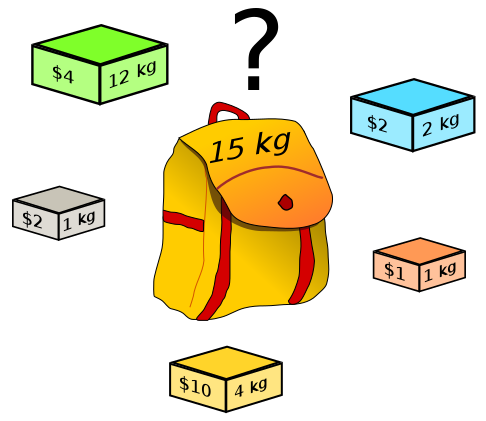
\includegraphics[scale=0.3]{fig/knapsack.png}
\end{figure}


\begin{block}{0-1 Knapsack}
  \begin{equation*}
    \begin{aligned}
      \text{maximize} & \quad \sum_{i=1}^{n} v_{i} x_{i} \\
      \text{subject to} & \quad \sum_{i=1}^{n} w_i x_{i} \leq W, \; \text{and} \; x_i \in \{0, 1\} 
    \end{aligned}
    \end{equation*}

\end{block}
\end{frame}


\begin{frame}{Knapsack Problem II}
 
\begin{block}{Multiple Knapsack}
  \begin{equation*}
    \begin{aligned}
      \text{maximize} & \quad \sum_{i=1}^{n} \sum_{j=1}^{m} p_{j} x_{ij} \\
      \text{subject to} & \quad \sum_{j=1}^{n} w_j x_{ij} \leq c_i, & i=1, \ldots, m, \\
      & \quad \sum_{i=1}^{m} x_{ij} \leq 1, & j = 1, \ldots, n \\
      & \quad x_{ij} \in \{0,1\}, & i=1, \ldots, m, \; j = 1, \ldots, n
    \end{aligned}
    \end{equation*}

\end{block}
\end{frame}


\begin{frame}{Modeling Toy Problem}

\begin{block}{Our Model}
  \begin{equation*}
    \begin{aligned}
      \text{\alert{minimize}} & \quad \sum_{i=1}^{n} \sum_{j=1}^{m} \alert{p_{ij}} x_{ij} \\
      \text{subject to} & \quad \sum_{j=1}^{n} w_j x_{ij} \leq c_i, & i=1, \ldots, m, \\
      & \quad \sum_{i=1}^{m} x_{ij} \alert{=} 1, & j = 1, \ldots, n \\
      & \quad x_{ij} \in \{0,1\}, & i=1, \ldots, m, \; j = 1, \ldots, n
    \end{aligned}
    \end{equation*}
\end{block}
  
\end{frame}


\begin{frame}[fragile]{Code - Models and Costs I}
  \scriptsize
  \begin{minted}[linenos]{python}
    import itertools
    from collections import namedtuple
  
    import sympy
  
    CostPerKg, Weight = sympy.symbols([ 'CostPerKg', 'Weight' ])

    ItemCost = CostPerKg * Weight
   
    Box = namedtuple('Box', ['weight'])
    Service = namedtuple('Service', ['capacity', 'cost_per_kg'])

  \end{minted}

\end{frame}


\begin{frame}{SymPy}
 \alert{SymPy} is a Python library for symbolic mathematics. 
 It aims to become a full-featured computer algebra system (CAS)
 while keeping the code as simple as possible in order to be comprehensible and easily extensible. 
 SymPy is written entirely in Python.
 
 Some Features:
       \begin{itemize}
        \item Construct expressions mathematically, \alert{\texttt{Piecewise}} function instead of \texttt{if ... elif ... then ... else}
	\item Latex output even in \alert{\texttt{jupyter}}
        \item Numeric computations, we can speedup with \alert{\texttt{numpy}} or  \alert{\texttt{Theano}}
        \item Autowrap module, code generation in \alert{\texttt{Fortran}} and \alert{\texttt{C}}
      \end{itemize}
 \begin{center}\url{sympy.org}\end{center}
\end{frame}

\begin{frame}[fragile]{SymPy - Piecewise example}

  \begin{minted}[linenos]{python}
   import sympy as sp
   from sympy.abc import x, y, z
   
   Condition = sp.symbols('Condition')
   
   expr = sympy.Piecewise(
      (x+1, Condition), 
      (x**2, sympy.Not(Condition)), 
      (0, True)
   )
   print(sympy.latex(expr))
   
  \end{minted}
\begin{center}
  \[
  expr = 
  \begin{cases}
    x + 1 & \text{for}\: Condition \\
    x^{2} & \text{for}\: \neg Condition \\
    0 & \text{otherwise}                                                                                    
  \end{cases}
  \]
\end{center}

\end{frame}


\begin{frame}[fragile]{Code - Models and Costs II}
  \[\text{minimize} \quad \sum_{i=1}^{n} \sum_{j=1}^{m} \alert{p_{ij}} x_{ij}\]

  \scriptsize
  \begin{minted}[linenos]{python}
      
    services = {
	'service1': Service(capacity=2.0, cost_per_kg=1.5),
	'service2': Service(capacity=10.0, cost_per_kg=0.9),
    }

    boxes = {
	'box1': Box(weight=1.0), 'box2': Box(weight=1.5),
	'box3': Box(weight=2.5), 'box4': Box(weight=6.5),
    }
	
    possible_assignments = list(itertools.product(boxes, services))
    
    # Calculate p_{ij} box_to_service costs
    b2s_costs = {}
    for box, service in possible_assignments:
	item_cost = ItemCost.subs({
	    'CostPerKg': services[service].cost_per_kg,
	    'Weight': boxes[box].weight
	})
	b2s_costs[box, service] = item_cost
  
  \end{minted}

\end{frame}


\begin{frame}[fragile]{Code - Optimization Model (Objective)}
  \[\text{\alert{minimize}} \quad \sum_{i=1}^{n} \sum_{j=1}^{m} p_{ij} \alert{x_{ij}}\]

  \scriptsize
  \begin{minted}[linenos]{python}
      import pulp
      
      model = pulp.LpProblem(
	  'Assignment Model', pulp.LpMinimize
      )
      
      # x_{ij}
      x = {
	  (b, t): pulp.LpVariable('b2s_%s_%s' % (b, t), cat=pulp.LpBinary)
	  for b, t in possible_assignments
      }
      
      model += sum([
	  x[box_to_service] * b2s_costs[box_to_service]
	  for box_to_service in possible_assignments
      ])
  \end{minted}
  
  
\end{frame}

\begin{frame}[fragile]{Code - Optimization Model (Constraints)}

\[ \sum_{j=1}^{n} w_j x_{ij} \leq c_i, \; \sum_{i=1}^{m} x_{ij} = 1, \; i=1, \ldots, m, \]

  \scriptsize
  \begin{minted}[linenos]{python}
      for service in services:
	  model += sum([
	      boxes[box_to_service[0]].weight * x[box_to_service]
	      for box_to_service in possible_assignments
	      if service in box_to_service
	  ]) <= services[service].capacity

      for box in boxes:
	  model += sum([
	      x[box_to_service]
	      for box_to_service in possible_assignments
	      if box in box_to_service
	  ]) == 1
  \end{minted}


\end{frame}

\begin{frame}[fragile]{Solve Model}

  \scriptsize
  \begin{minted}[linenos]{python}
   import PrettyTable
  
   solver = pulp.PULP_CBC_CMD(msg=1)
   status = model.solve(solver)
   
   prettytable = PrettyTable(['Service', 'Capacity', 'Boxes'])
   ...
   print(prettytable)
  \end{minted}

    \begin{table}

    \caption{Results I}
    \begin{tabular}{lcc}
     \toprule
     Service & Capacity (kg) & Boxes \\
     \midrule
     UFS & 2.0 & box2(1.5) \\
     FedRex & 10.0 & box1(1.0), box3(2.5), box4(6.5) \\
     \bottomrule
    \end{tabular}

  \end{table}
  
\end{frame}

\begin{frame}{Real Problem}

\begin{itemize}

\item Minimize the total cost of production
\item Choose press sheets from press sheet templates
\item Choose which orders to print on each press sheet
\item Choose presses to print each press sheet
\item This decision is made daily.
\item Products that are due today must be printed.
\item Products not due today may optionally be printed.
\end{itemize}
 
\end{frame}


\begin{frame}{Press Sheet Templates I}
 
\begin{figure}
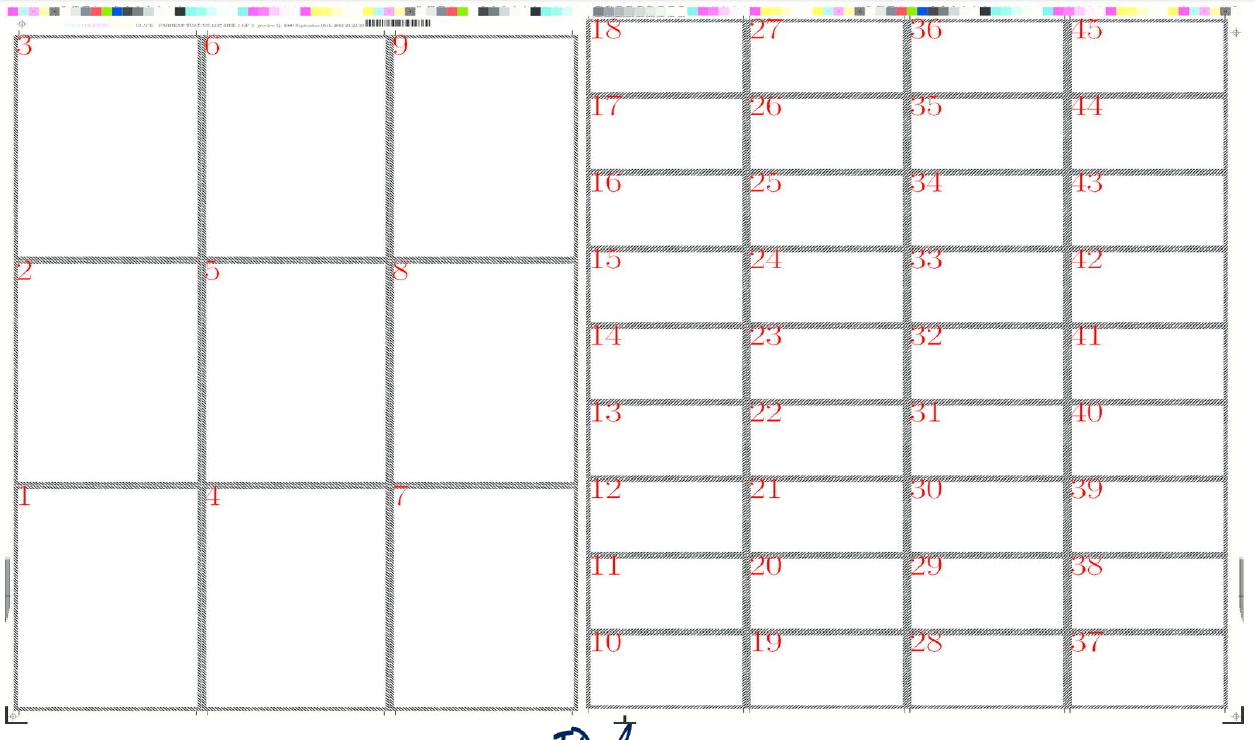
\includegraphics[scale=0.3]{fig/template1.png}
\end{figure}

\end{frame}

\begin{frame}{Press Sheet Templates II}
 
\begin{figure}
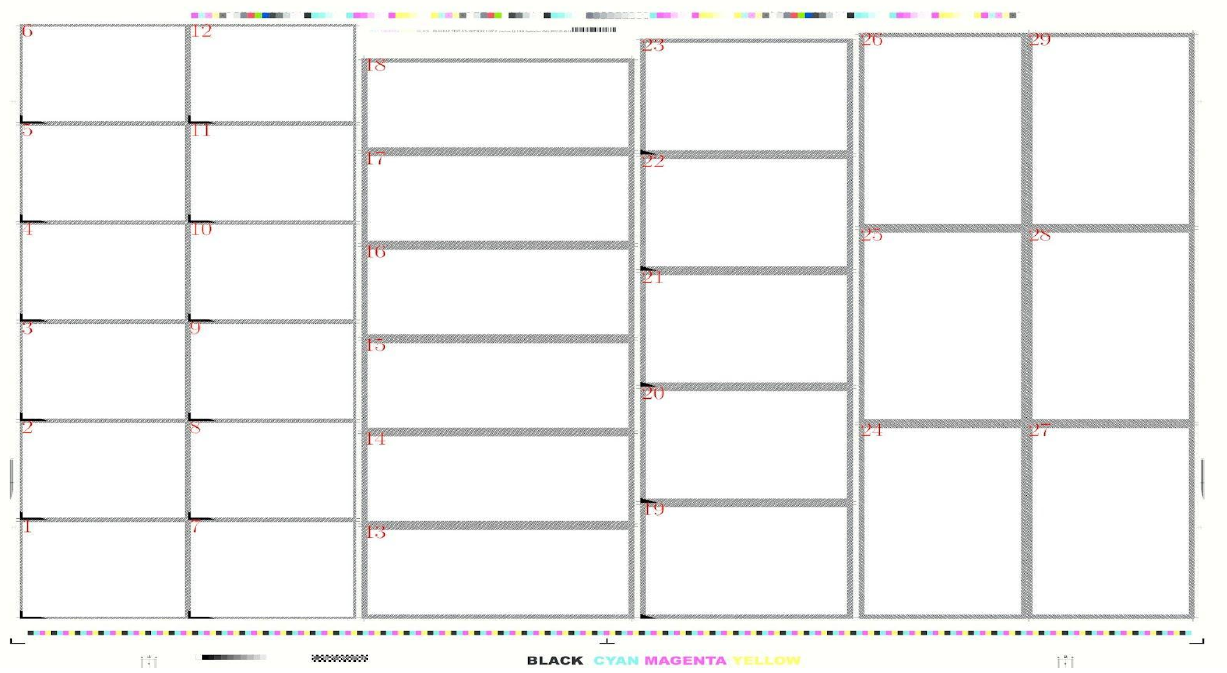
\includegraphics[scale=0.3]{fig/template2.png}
\end{figure}

\end{frame}


\begin{frame}{Costs Model}
 \begin{itemize}
  \item Paper Cost
  \item Plate Cost
  \item Ink Cost
  \item Press Time / Press Labor Cost
  \item UV Spot and Full Cost / UV Labor Cost
  \item Cutting Time / Cutting Labor Cost
  \item Cost tradeoffs due to press sheet type, press,
    quantity, labor, etc.

 \end{itemize}

\end{frame}

\begin{frame}{Order Placement Complexity}

\begin{itemize}
 \item Orders can be placed multiple times on each press
sheet.
 \item Orders can be split across multiple press sheets
 \item Orders can be “over-printed”
 \item 1-sided orders may be placed on 2-sided press sheets
 \item “UV Full” coated orders may be placed on “UV Spot”
press sheets

\end{itemize}


\end{frame}

\begin{frame}{Optimization Model}

\begin{figure}
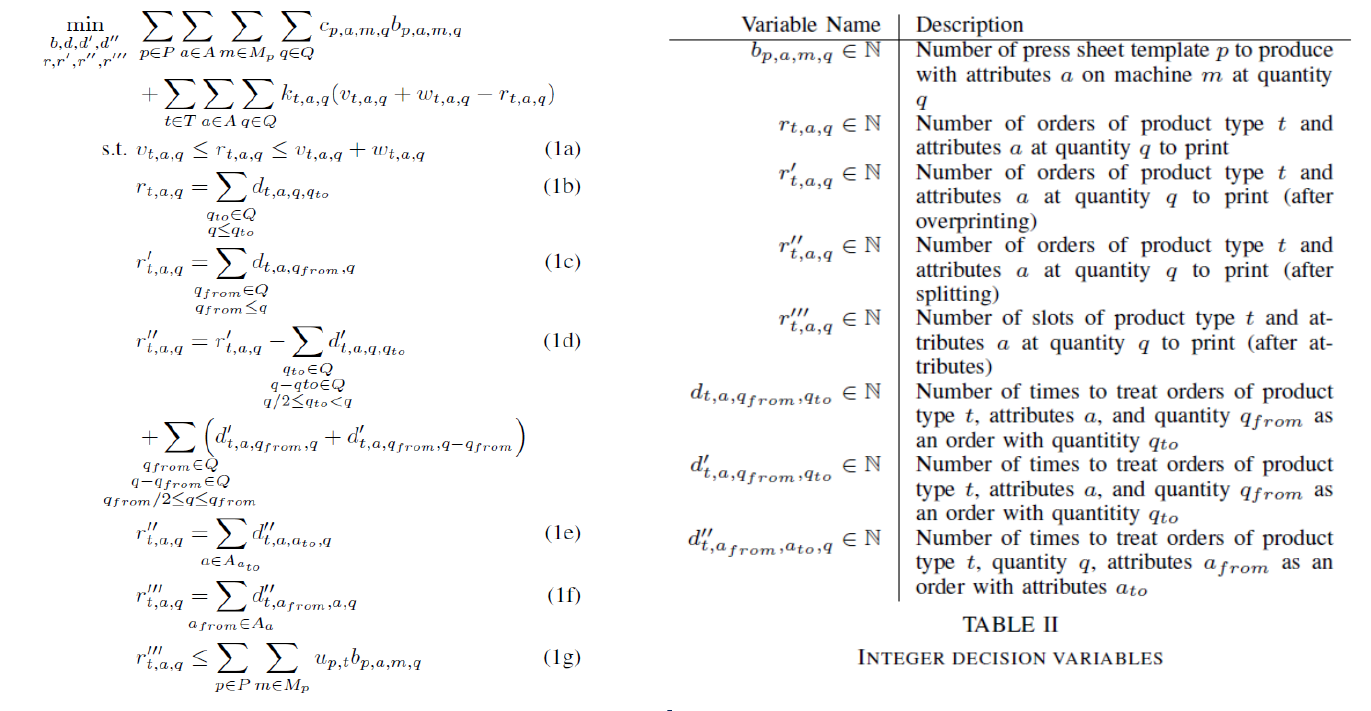
\includegraphics[scale=0.3]{fig/opt_problem.png}
\end{figure}

\end{frame}



\begin{frame}{References}

 \begin{thebibliography}{9}

\bibitem{shyman05}
  Jan A. Shyman,
  \emph{Practial Mathematical Optimization - An Introduction to Basic Optimization Theory and Classical and New Gradient-Based Algorithms},
  Springer,
  2005.

\bibitem{pisinger95}
  David Pisinger,
  \emph{Algorithms for Knapsack Problems},
  Ph.D. thesis, 1995.

\bibitem{fullmer13}
  Daniel Fullmer, Sean Warnick,
  \emph{Press Sheet Optimization for Open Loop Control of Industrial Scale
Gang-Run Printing},
  2013
  
\end{thebibliography}
\end{frame}


\end{document}
